\documentclass[english,a4paper,oneside]{article}
\usepackage{babel}	
\usepackage{amsmath}
\usepackage{amssymb}
\usepackage{mathrsfs}
\usepackage{mathtools}
\usepackage[utf8]{inputenc}
\usepackage[T1]{fontenc}	
\usepackage{graphicx}		
\usepackage{dcolumn}		
\usepackage{booktabs}		
\usepackage{eurosym}
\usepackage{siunitx}
\usepackage{amsthm}
%\usepackage{algorithm}
%\usepackage{algpseudocode}
\usepackage{verbatim}
\usepackage{natbib}
%\usepackage{minted} % Code typesetting
\usepackage{multirow}
\usepackage{blkarray} %Block matrix display
\usepackage{todonotes}
\usepackage{cleveref}
\usepackage{caption}
\usepackage{listings}
%\usepackage{fullpage}
\usepackage{marginnote}
\usepackage[top=1.5cm, bottom=1.5cm, outer=5cm, inner=2cm, heightrounded, marginparwidth=2.5cm, marginparsep=2cm]{geometry}

\newcommand{\element}[3]{$^{#2}_{#3}\mathrm{#1}$}
\newcommand\up[1]{\ensuremath{\textup{#1}}}
\newcommand\dd{\ensuremath{\textup{d}}}
\newcommand{\avg}[1]{\left< #1 \right>}
\newcommand{\Var}[1]{\up{Var}}
\DeclareMathOperator{\erf}{erf}

\newtheorem{mytheorem}{Theorem}
\newtheorem{mydefinition}{Definition}


%%%%%
%  GAMS Markup in listings enviroment
%%%%%

\lstdefinelanguage{GAMS}{
morekeywords={
ABORT, ACRONYM, ACRONYMS, ALIAS, ALL, AND, ASSIGN, BINARY, CARD, DISPLAY, EPS, EQ, EQUATION, EQUATIONS, GE, GT, INF, INTEGER, LE, LOOP, LT, MAXIMIZING, MINIMIZING, MODEL, MODELS, NA, NE, NEGATIVE, NOT, OPTION, OPTIONS, OR, ORD, PARAMETER, PARAMETERS, POSITIVE, PROD, SCALAR, SCALARS, SET, SETS, SMAX, SMIN, SOS1, SOS2, SUM, SYSTEM, TABLE, USING, VARIABLE, VARIABLES, XOR, YES, REPEAT, UNTIL, WHILE, IF, THEN, ELSE, SEMICONT, SEMIINT, FILE, FILES, PUT, PUTPAGE, PUTTL, PUTCLOSE, FREE, NO, SOLVE, FOR, ELSEIF, ABS, ARCTAN, CEIL, COS, ERROR, EXP, FLOOR, LOG, LOG10, MAP, MAPVAL, MAX, MIN, MOD, NORMAL, POWER, ROUND, SIGN, SIN, SQR, SQRT, TRUNC, UNIFORM, LO, UP, FX, SCALE, PRIOR, PC, PS, PW, TM, BM, CASE, DATE, IFILE, OFILE, PAGE, RDATE, RFILE, RTIME, SFILE, TIME, TITLE, TS, TL, TE, TF, LJ, NJ, SJ, TJ, LW, NW, SW, TW, ND, NR, NZ, CC, HDCC, TLCC, LL, HDLL, TLLL, LP, WS, /,PROD: },
sensitive = false,
morecomment=[f]*,%
morecomment=[s]{\$ontext}{\$offtext},
%morecomment=[s][\color{green}]{/}{/},
morestring=[b]“,
morestring=[b]‘
}
\lstset{
basicstyle=\fontfamily{pcr}\fontseries{m}\selectfont\footnotesize,
commentstyle=\color{gray}\itshape,
keywordstyle=\color{blue}\bfseries,
stringstyle=\color[rgb]{0.5,0,0.5}\itshape,
showstringspaces=false,
numbers=left,
numberstyle=\color[rgb]{0,0.5,0.5}\fontfamily{pcr}\fontseries{m}\selectfont\tiny,
numberblanklines=false,
showlines=false,
belowskip=\bigskipamount{},
breaklines=true,
%stepnumber=2,
tabsize=6,
%extendedchars=true,
%float=h,
frame=tb
}


\raggedbottom{}
%\parindent = 0pt

\begin{document}

\title{Exam Project 1: Asset Liability Management in a pension fund}
\author{Tue Vissing Jensen, DTU Elektro\footnote{tvjens@elektro.dtu.dk}
		\and Tiago Soares, DTU Elektro\footnote{tiasoar@elektro.dtu.dk}}
\date{\today}
\maketitle

\section{Nomenclature}
\begin{description}
\item[$t \in T = {0, \ldots, \tau}$]{Time steps, measured relative to current year.}
\item[$i \in E$]{ETF index}
\item[$m \in M$]{Months subset index of $T$}
\item[$T_m \subset T$]{Specified interval dates}
\item[$s \in \Omega$]{Scenarios index}
\item[$st \in ST$]{Index over weeks included in monthly scenarios}
\item[$P_{i,t}$]{Price of ETF $i$ at time $t$}
\end{description}



\section{Data download and clustering analysis}

Price data on the ETFs is downloaded from Google Finance using the data download functionality built in to the Pandas module for Python.
We use the closing price of the ETF for each day to represent the day's price.
Any ETF with less than 2400 data points is excluded, leaving 93 of the initial 100 ETFs to use for further processing.

To cluster the data, it is necessary to define a distance between assets. We compute the correlation coefficient $C_{ij}$ between assets $i$ and $j$, and define the distance between them as
\begin{gather}
d(i,j) = 1 - C_{ij}^2  \in [0, 1].
\end{gather}
This distance will tend to group together assets that are more correlated and/or anti-correlated together.
This is intuitively a reasonable measure, as (1) going long on an asset is the same as going short on an asset that is anti-correlated with it, and we wish to treat short and long assets the same in this analysis, and (2) the difference between a correlation of 1.00 and 0.95 is more significant than between 0.05 and 0.00.


\begin{figure}[tp]
\centering
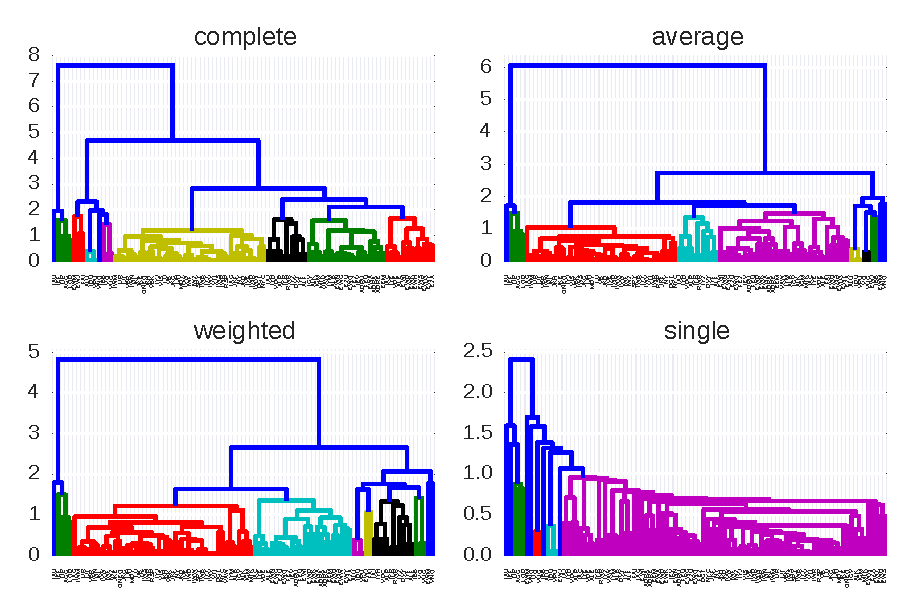
\includegraphics{pic/dendro_methods.pdf}
\caption{DELETE ME IN FINAL:\ Dendrogram of clustering found by various methods. All non-blue leaves are trimmed by the max-mean and the min-std criteria.}
\label{fig:bondsyield}
\end{figure}

\begin{figure}[tp]
\centering
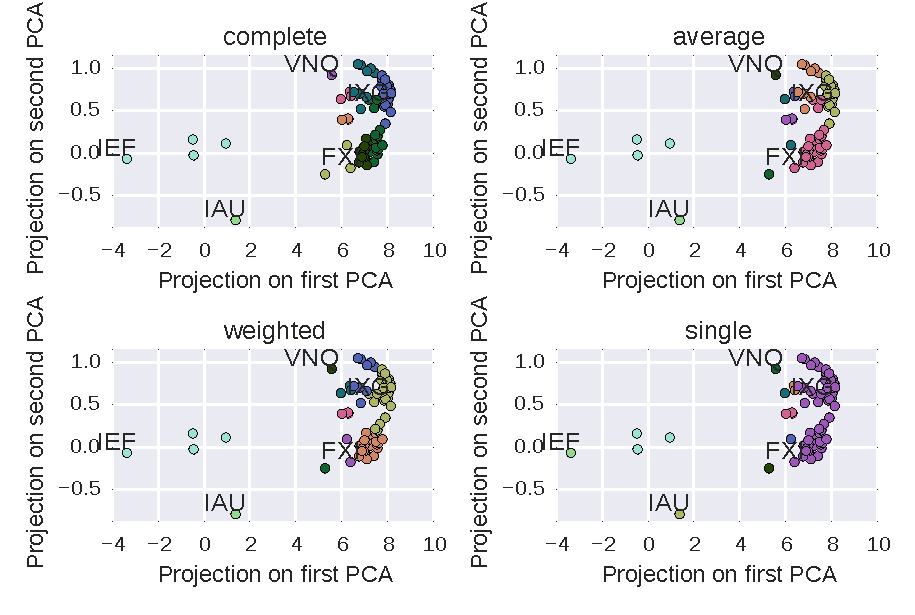
\includegraphics{pic/pca_methods.pdf}
\caption{Projection of asset correlation onto the largest principal components. These account for 78.58\% and 4.51\% of the variance, respectively.}
\label{fig:bondsyield}
\end{figure}


\section{Scenario generation}

The period of study considered in this work is  between 02/02/2005 and 12/11/2014, with the aim to produce a back-test starting on 27/02/2008.
In order to generate scenarios to be used for CVaR model, several assumptions are needed. The historical return for each ETF over the period $t$ is given by
\begin{gather}
r_{i,t} = \frac{P_{i,t+1}}{P_{i,t}}-1, \;\; \forall i \in E, t \in T
\end{gather}
The scenarios are randomly generated picking four dates in a specified interval and taking the historical returns for the ETF's as
\begin{gather}
WRS_{i,st,s,m} = r_{i,t}  \up{ for } t \equiv RANDOM(T_{m}), \;\; \forall i \in E, st \in ST, s \in \Omega, m \in M
\end{gather}
where $WRS_{i,st,s,m}$ is the weekly return scenarios for each month $m$.
The first specified interval$T_1$ where is picked the historical returns is between 28/01/2005 and 27/02/2008.
For each $m$ the specified interval shift itself one month until the end of the period of study (12/11/2014).
The monthly return for each of scenario $MRS_{i,s,m}$ is based on accumulating the four weeks return scenario and is determined as
\begin{gather}
MRS_{i,s,m} = \prod_{st} (1+WRS_{i,st,s,m}) -1, \;\; \forall i \in E, s \in \Omega, m \in M
\end{gather}


\section{Optimal portfolio strategy}

WORDS

\section{Comparison with 1/N strategy}

In the $1/N$ strategy, on the first trading day we invest  an equal amount into each asset, and then leave the assets be for the entire trading period.

Since we are investing into 10 assets at a cost of 0.1\% of the trading volume, it costs us 1000 DKK to make the initial trade.
The remaining 999.000 DKK are left to grow during the entire period.

This strategy yields an annualized return of 5.7\% for the max-mean assets, and of 2.4\% for the min-stdev.


\begin{figure}[tp]
\centering
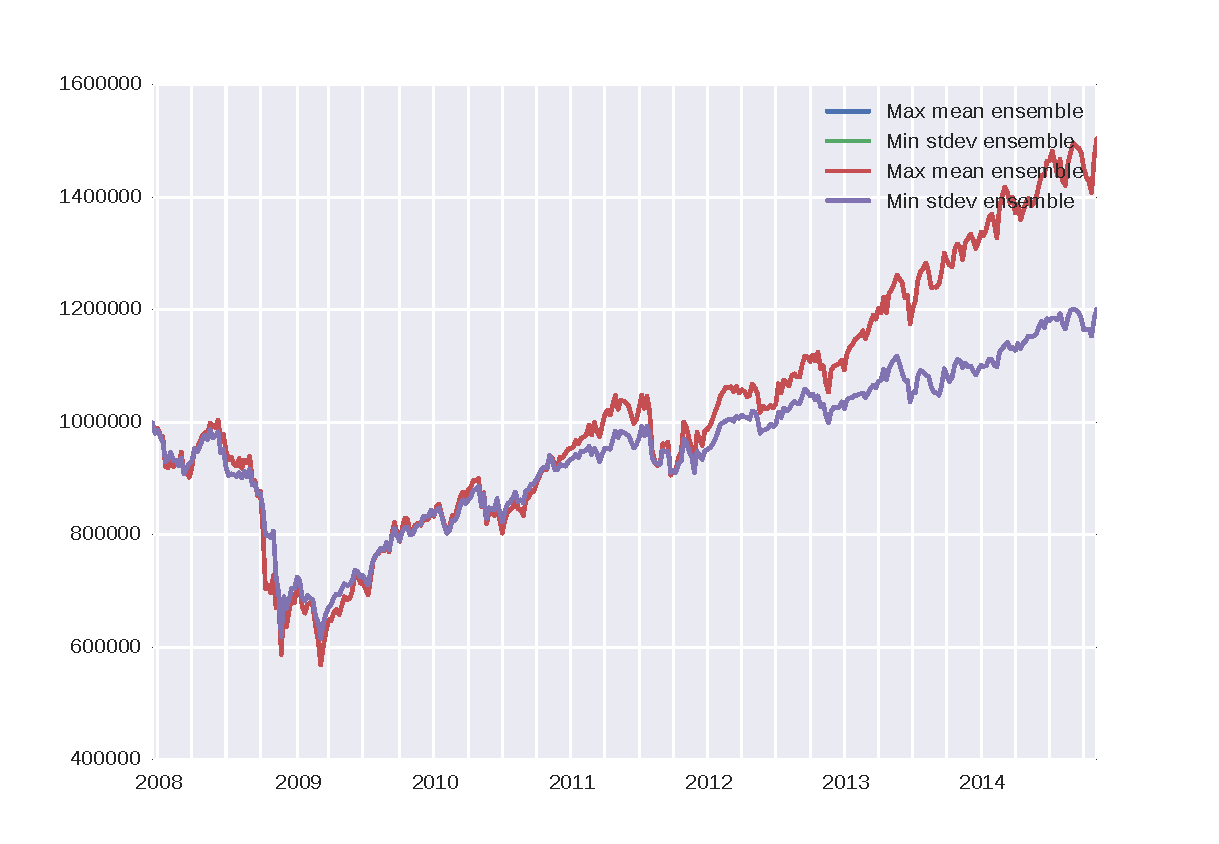
\includegraphics{../pic/returns_1overN_only.pdf}
\caption{DELETE ME IN FINAL:\ Returns for the 1/N strategy for the ensembles indicated.}
\label{fig:bondsyield}
\end{figure}


\clearpage

\appendix

\section{Gams code\label{sec:appendixcode}}

All code from this project is available at \url{www.github.com/TueVJ/OptFinFinalExam}~.


\begin{align}
\underset{r_t}{\min} \; \; & (1 - \lambda) \sum_i {\left( P_i - \sum_t \frac{F(i,t)}{{(1+r_t)}^t} \right)}^2  \label{eq:objweighted}\\
& + \lambda \sum_t {\left(f_{t(t-1)} - f_{(t-1)(t-2)}\right)}^2 \nonumber \; .\\
\end{align}

\begin{figure}[tp]
\centering
%\includegraphics{img/bondsyield.pdf}
\caption{Caption Here}
\label{fig:bondsyield}
\end{figure}


\end{document}

